\section{DNA and molecular barcoding}

\subsection{History and application}

Analogous to the Universal Product Codes (UPCs) found on commercial goods, genetic barcodes are created through the amplification and sequencing of short segments or gene regions of an organism\textsc{\char13}s genome - most commonly the mitochondrial cytochrome oxidase I (COI) gene in animals, and the chloroplast rbcL (RuBisCo large subunit) and matK (maturase k) loci in plants \citep{Hebert2003, CBOL2009, Floyd2010}. These unique signature sequences are used for identification and for phylogenetic analyses \citep{Hebert2003}. Mitochondrial genes are the preferred targets for barcoding initiatives due to their generally higher mutation rates compared to nuclear genes \citep{Drake1998, Ballard2004, Haag-Liautard2008}, their relatively low rates of recombination \citep{Piganeau2004}, and their high abundance in cells \citep{Waugh2007}. The COI marker is particularly useful because it displays low rates of insertions and deletions, and despite being a relatively conserved region, it can be used to differentiate between species; particularly in insects \citep{Hebert2003, Blaxter2004}. 
Although the concept of species identification using molecular techniques began in the 1980s, particularly regarding microorganisms \citep{Nanney1982, McAndrew1983, Anderson1985}, \citet{Arnot1993} first used the term `DNA barcode' in a study aiming to barcode isolates of the \textit{Plasmodium falciparum} Welch protozoan. The method gained popularity in 2003 \citep{Hebert2003, Hebert2003a}, and the Consortium for the Barcode of Life (CBOL) was founded the following year \citep{CBOL2009}. The Barcode of Life Database (BOLD) currently contains over 6 million genetic barcodes representing 215 000 animal, 69 000 plant, and 22 000 fungal species \citep{BOLD2019}.
Also referred to as `microgenomic identification', genetic barcoding relies on nucleotide diversity between organisms to group them taxonomically, or according to distinct haplotypes \citep{Hebert2003a}. It is based on the premise that interspecific variation is greater than intraspecific variation, referred to as the `barcoding gap' \citep{Hebert2003}. An arbitrary sequence divergence criterion suggested that species could be delineated at 3\% for insects, and 2\% and above for vertebrates \citep{Hebert2003}. 
DNA barcoding can serve as an efficient tool for taxonomists, and has a wide variety of cross-disciplinary applications \citep{Savolainen2005, Frezal2008, Valentini2008} (see Table \ref{tab:barcoding}).
A major advantage of genetic barcoding is its applicability to various stages of an organism's life cycle; as the genetic signature remains the same irrespective of differences in the individual's age \citep{Floyd2010}. 

\subsection{Caveats}

Despite the advantages, there are a number of criticisms of DNA barcoding, particularly with reference to its use as a standalone tool for the description of new species \citep{Rubinoff2006a}. The main arguments put forward include the the following: \vspace{0.4cm}
% \citet{Moritz2004DNAPitfalls, Will2004MythClassification,Rubinoff2005BetweenInference,Will2005,Cameron2006, Rubinoff2006, Rubinoff2006a, Frezal2008, Valentini2008, Pecnikar2014}. \\

\begin{enumerate}
    \item Heteroplasmy and differential inheritance of mitochondrial genomes.
    \item Maternal mitochondrial inheritance.
    \item Differential rates of gene evolution.
    \item Introgression of mitochondrial genes.
    \item Incomplete lineage sorting.
    \item The occurrence of nuclear mitochondrial DNA segments (numts).
\end{enumerate}

\subsubsection{Heteroplasmy}
Heteroplasmy in the mitochondrial genome refers to the presence of more than one genotype within an organism, such that there is a ratio of `mitotypes' (analogous to haploptypes); where one is often predominant over the others \citep{Kmiec2006}. Mitotypes can come about due to differences in nucleotide length (length heteroplasmy) or composition of mtDNA (site heteroplasmy) due to the insertion or deletion of large fragments, or errors in the replication process \citep{Barr2005}. New mitotypes can also be created following the exposure of mtDNA to oxygen metabolites, resulting in point mutations \citep{Kmiec2006}. Mitochondria are the vestiges of ancestral bacterial endosymbionts \citep{Gray1999} and replicate independently of the nucleus \citep{Meusel1993}. This unique system of genomic segregation and replication results in the differential transferal of mitochondrial genomes to daughter cells; facilitating heteroplasmy \citep{Barr2005}. 

\subsubsection{Maternal inheritance}
Although mitochondrial genomes are predominantly maternally inherited and rarely undergo recombination in animals, there are an increasing number of cases of biparental inheritance, or `paternal leakage', in which some mitochondrial sequences are inherited from males \citep{Gyllensten1991, Zouros1992, Skibinski1994, Hoarau2002, Kvist2003, Barr2005, Xiong2013, Ladoukakis2017}. This has been found in some insects, such as \textit{Drosophila simulans} Sturtevant (Diptera: Drosophilidae) \citep{Wolff2013} and \textit{Magicicada} spp. L. (Hemiptera: Cicadidae) \citep{Fontaine2007}. Additionally, `doubly uniparental inheritance' is another system that is common in bivalves, where male offspring inherit mtDNA from both parents while females inherit maternal mtDNA only \citep{Zouros1994}. The paternal transmission of mtDNA is usually prevented through a number of mechanisms across species, such as the destruction of male mitochondria in the developing zygote, the total absence of mitochondria in sperm, and the prevention of male mitochondria entering the oocyte upon fertilisation \citep{Rokas2003}. The process of paternal leakage, however, occurs more frequently in animals than was previously realised and can contribute to inconsistencies in the comparison of genetic barcodes. This is in addition to the growing understanding of the effects of mitochondrial bottlenecks during oogenesis \citep{Jenuth1996, Stewart2008} and the occurrence of mitochondrial recombination in some animals \citep{Piganeau2004, Rubinoff2006a}. \\
Since mitochondrial genomes are predominantly maternally inherited, the resulting sequences may be sex-biased \citep{Rubinoff2006a, Frezal2008, Innocenti2011}. Selection pressures that differentially affect males and females are therefore not taken into account, such as differences in motility \citep{Rubinoff2004}, feeding preference \citep{Hulcr2007}, and the occurrence of genetic diseases \citep{Frank1996, Camus2012}. Additionally, the barcoding of insects infected with \textit{Wolbachia} bacteria might lead to inaccuracies due to the effect that the symbionts have on reproductive functioning and the transferal of mitochondrial haplotypes in a population \citep{Gerth2011}. 

\subsubsection{Differential rates of gene evolution}
Analogous to the uncertainties of the differential rate of mutation in the use of molecular clocks \citep{Penny2005, Pulquerio2007, Weir2008}, the rate of evolution in the genes used for barcoding will vary between taxonomic groups \citep{Rubinoff2006a}. Mutation rates of genes in mitochondria are influenced by the unique asymmetrical mode of replication of the genome, where proximity to the site where replication begins is important \citep{Gibson2004}. The lagging strand remains single-stranded until about two thirds of the leading strand has been replicated, which renders it more susceptible to mutations \citep{Clayton2003, Rubinoff2006}. Genome arrangements are not necessarily consistent across taxonomic groups owing to the vast array of genetic systems in existence, and to factors such as life history strategies \citep{Rubinoff2006}. 
This could affect genetic barcoding through the size of the resulting barcode gap. A small or negative barcode gap results when there are too few mutational differences between groups to be able to tell them apart.

\subsubsection{Introgression of mitochondrial genes}
Introgression, also referred to as interspecific gene flow, is the incorporation of genes from the gene pool of one species into that of another through hybridisation and backcrossing \citep{Funk2003, Harrison2014}. This leads to polyphyly and the incongruence between gene and species trees \citep{Funk2003, Petit2009}. The introgression of mitochondrial genes used in barcoding initiatives can result in misleading conclusions, as taxonomic boundaries can become blurred \citep{Rubinoff2006, Petit2009, Ermakov2015}.
Mitochondrial introgression is particularly problematic due to limited recombination, resulting in the persistence of introgressed gene regions in a genome \citep{Funk2003}. An important assumption in analysing intra-and interspecific variation is that the study species are monophyletic with regards to the gene region of interest \citep{Funk2003}. \\
A number of studies have found that COI barcodes [alone] were unable to distinguish between species due to potential mitochondrial introgression and/or incomplete lineage sorting, such as in some cave-dwelling spiders (\textit{Circurina} spp.) (Araneae: Dictynidae) \citep{Paquin}, ground beetles (\textit{Carabus} L.) spp. (Coleoptera: Carabidae) \citep{Sota2001, Raupach2010}, African fruit bats (\textit{Pteropodidae} Gray) \citep{Nesi2011}, swallowtail butterflies (\textit{Papilio machaon} L.) (Lepidoptera: Papilionidae) \citep{Sperling1994}, and hairstreak butterflies (\textit{Calycopis} Scudder spp.) (Lepidoptera: Lycaenidae) \citep{Cong2017}. 

\subsubsection{Incomplete lineage sorting}
As with introgression, incomplete lineage sorting (or `deep coalescence') results in inconsistencies in topology between gene and species trees, such that the phylogeny of a particular gene does not match that of the species as a whole \citep{Maddison1997, Nichols2001,Funk2003}. Incomplete lineage sorting occurs when the coalescence of a gene back to a common ancestor pre-dates the speciation event (Fig. \ref{fig:gene_tree}) \citep{Maddison1997}. As such, the `sorting' of genes into the bifurcating lineages is not yet complete. 

\begin{figure}[H]
	\centering
	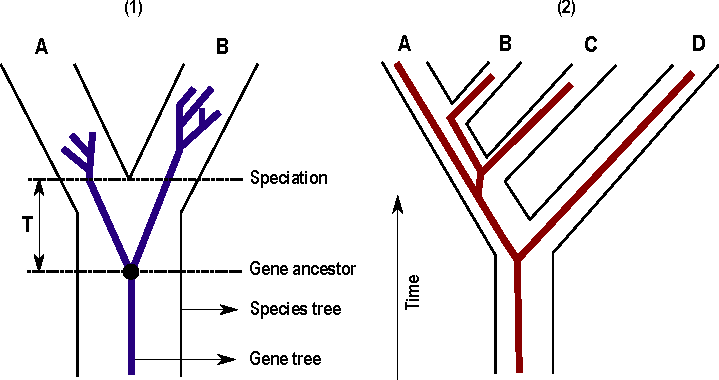
\includegraphics[scale = 1]{Images/gene_trees.pdf}
    \newline
	\caption{Gene trees within species trees, illustrating deep coalescence. (1) shows how the most recent common ancestor in the gene tree pre-dates that of the species tree by time T. (2) is another example of how the topology of a gene and species tree can differ. The species tree suggests that A and B share the most recent common ancestor, while the gene tree contrastingly shows that this is true for B and C. (Adapted from \citet{Maddison1997,Nichols2001,Edwards2009}).}
	\label{fig:gene_tree}
\end{figure}

\subsubsection{Nuclear mitochondrial DNA segments}
Nuclear mitochondrial DNAs (`numts'), also referred to as `pseudogenes', are non-functional gene regions that have translocated from the mitochondrial to the nuclear genome \citep{DErrico2004, Frezal2008, Hazkani-Covo2010, Leite2012}. Pseudogenes were first discovered in mice \citep{DuBuy1967} and locusts (\textit{Locusta migratoria} L.) (Orthoptera: Acrididae) \citep{Gellissen1983}, and have since been found to occur frequently across a wide range of taxa \citep{Lopez1994, Zhang1996, Williams2001, Richly2004, Pamilo2007}; particularly in plants and arthropods \citep{Gellissen1983, Bensasson2000, Bensasson2001, Buhay2009}. One of the most extreme examples was found in the domestic cat, where nearly half of its mitochondrial genome was present in the nucleus \citep{Lopez1994}! It is believed that the transfer of mitochondrial genes to the nucleus is a very ancient process, and that pseudogenes might arise due to unsuccessful transfers between the two organelles \citep{DErrico2004}. 
Pseudogenes are problematic in DNA barcoding because these regions can be co-amplified in addition to the target mitochondrial gene (identifiable by differences in nucleotide composition, the presence of indels, point mutations, and in-frame stop codons) \citep{Bensasson2001, Song2008, Moulton2010, Ahmed2015}. Depending on the accumulation of mutations (where mutation rates and selection pressures differ between the mitochondrial and nuclear genomes), conservative primers may preferentially amplify pseudogenes, resulting in paralogous sequences that have little comparative value and lead to the inference of incorrect phylogenetic relationships \citep{Bensasson2001, Song2008, Moulton2010, Leite2012}. To further complicate matters, the number of copies and composition of pseudogenes can vary between individuals, where multiple independent transferral events could have occurred over time \citep{Bensasson2000,Bensasson2001}. \citet{Song2008} found that the presence of pseudogenes in the COI barcodes for grasshoppers and crayfish lead to an overestimation of the number of species sampled by 2.8 and 3.6-fold, respectively. The authors concluded that the co-amplification of pseudogenes can be `disastrous' for DNA barcoding if sequences are not screened properly, and if only one gene marker is relied upon. \\
Despite the potential shortcomings of barcoding, the method has been successfully applied in numerous studies involving insects, representing groups such as the Heteroptera \citep{Raupach2014, Havemann2018}, Orthoptera \citep{Hawlitschek2017}, Lepidoptera \citep{Hausmann2013GeneticSystem, Razowski2017UncoveringTortricidae, Spitsyn2018DNAPleistocene}, Coleoptera \citep{Raupach2010, Hendrich2015ABOLD}, Diptera \citep{Lin2015ExploringBarcodes}, Ephemeroptera, Plecoptera, Trichoptera \citep{Cordero2017DNACanada,Cukusic2017DNACroatia}, and Hymenoptera \citep{Schmidt2017IdentificationCaveats}. If used appropriately, while remaining cognisant of its weaknesses, genetic barcoding can serve as a very valuable identification tool.